\documentclass{article}
\usepackage{amsmath, amssymb, amsthm}
\usepackage{newtxtext,newtxmath}
\usepackage{graphicx}
\usepackage{caption}
\usepackage{subcaption}

\graphicspath{ {../images/} }

\title{Removing Projective Distortion from Images}
\author{Mickey Smith}
\date{August 2019}

\begin{document}

\maketitle

\section{Homogenous Coordinates}
Similar to cartesian coordinates, homogenous coordinates are a way to represent points in a given dimension.

\begin{figure}[hbt!]
\centering
\begin{subfigure}{.5\textwidth}
    \centering
    \begin{pmatrix}
        x \\
        y
    \end{pmatrix}
    \caption{Cartesian $\mathbb{R}^2$}
    \label{fig:coords_sub1}
\end{subfigure}%
\begin{subfigure}{.5\textwidth}
    \centering
    \begin{pmatrix}
        x \\
        y \\
        1
    \end{pmatrix}
    \caption{Homogenous $\mathbb{R}^2$}
    \label{fig:coords_sub2}
\end{subfigure}
\caption{Representing coordinates as homogenous and cartesian}
\label{fig:coords}
\end{figure}

The only practical difference between cartesian and homogenous representations for the purposes of this assignment is that homogenous coordinates contain an extra dimension value that represents vector scaling. This allows a point to be further from the origin on its component vector without altering the other coordinates.

\clearpage
\section{Projective Transformations}
When a photo is taken of a scene, the camera applies a homography to the original scene, creating a new perspective captured by the photo. An original scene \( \textbf{x} \) manipulated by a photo becomes \( \textbf{x}' \) through the application of projective homography \( H \).

\begin{figure}[h]
    \centering
    \( \textbf{x}' \) = \( H\textbf{x} \)
    \caption{Homography application}
\end{figure}

This equation is notably of the form \( Ax = B \), which will allow us to solve for the homography matrix easily.

This means that in order to restore the original image's perspective, we need to determine \( H^{-1} \). Once we have \( H^{-1} \) we can apply it to every pixel location in the image and determine its location in a new image.

In order for a program to apply these inverse transformations, 8 coordinates within $\mathbb{R}^2$ have to be defined. 4 representing the corners of a box within the supplied image and 4 representing the destination location of those points within the new image. We'll choose those locations as the corners of a rectangle within the image.

\begin{figure}[h]
\centering
\begin{subfigure}{.5\textwidth}
    \centering
    \begin{pmatrix}
        \( x^{ll} \) \\
        \( x^{lr} \) \\
        \( x^{ul} \) \\
        \( x^{ur} \)
    \end{pmatrix}
    \caption{Image points}
    \label{fig:coords_sub1}
\end{subfigure}%
\begin{subfigure}{.5\textwidth}
    \centering
    \begin{pmatrix}
        \( x^{'ll} \) \\
        \( x^{'lr} \) \\
        \( x^{'ul} \) \\
        \( x^{'ur} \)
    \end{pmatrix}
    \caption{World points}
    \label{fig:coords_sub2}
\end{subfigure}
\caption{Image and world point definitions}
\label{fig:coords}
\end{figure}

For i in all 4 corners:

\begin{figure}[h]
    \centering
    \begin{gather}
        \begin{pmatrix}
            \( x^{i} & y^{i} & 1 & 0 & 0 & 0  & -x^{i}x^{'i} & -x^{i}y^{'i} \) \\
            \( 0 & 0 & 0 & x^{i} & y^{i} & 1 & -y^{'i}x^{i} & -y^{'i}y^{i} \)
        \end{pmatrix}
        \begin{pmatrix}
            \( h_{1} \) \\
            \( h_{2} \) \\
            \( h_{3} \) \\
            \( h_{4} \) \\
            \( h_{5} \) \\
            \( h_{6} \) \\
            \( h_{7} \) \\
            \( h_{8} \) \\
            \( h_{9} \)
        \end{pmatrix}
        =
        \begin{pmatrix}
            \( x^{'i} \) \\
            \( y^{'i} \)
        \end{pmatrix}
    \end{gather}
    \caption{Homography application}
\end{figure}

\begin{figure}[hbt!]
    \centering
    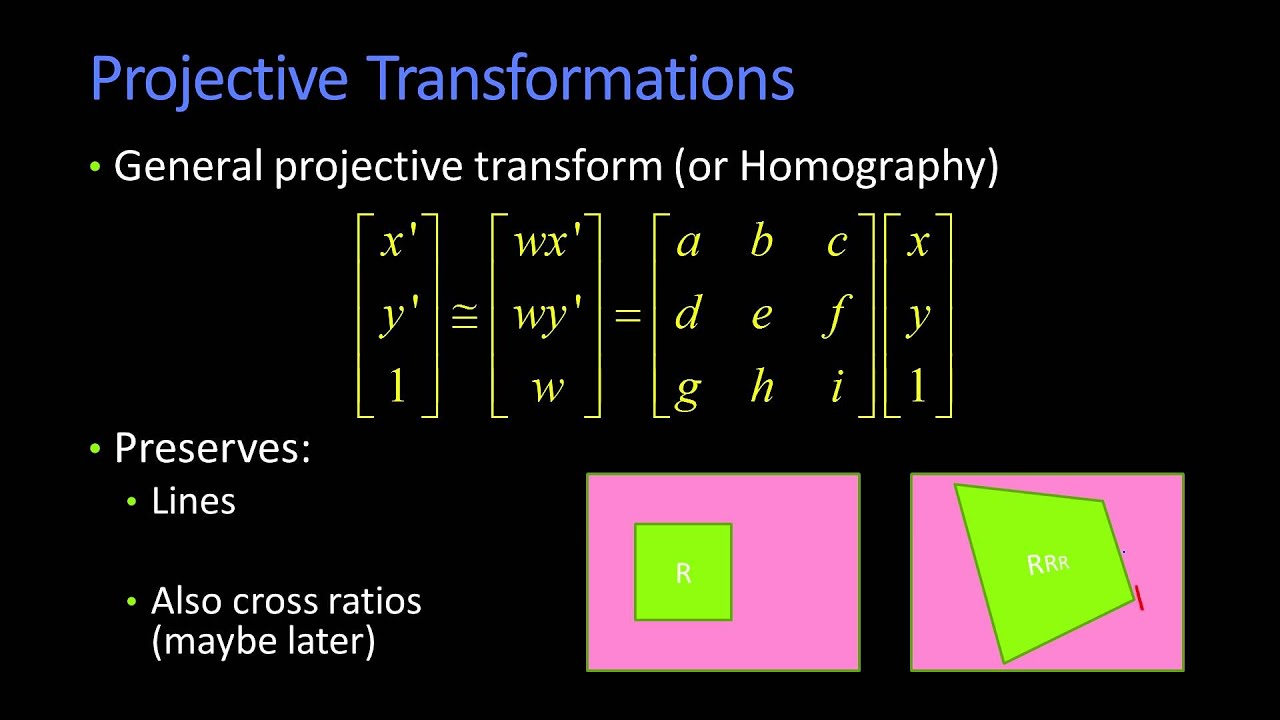
\includegraphics[scale=0.2]{projective_transform}
    \caption{Explanation of projective transforms}
\end{figure}

\end{document}
